%   Filename    : chapter_4.tex 
\chapter{Preliminary Results/System Prototype}
\section{Data Gathering}
The data for dengue case prediction was gathered from a variety of reliable sources, enabling a comprehensive dataset spanning from January 2016 to September 2024. This dataset includes 452 rows of data, each containing weekly records of dengue cases along with corresponding meteorological variables, such as rainfall, temperature, and humidity.
\begin{enumerate}
	\item Dengue Case Data: The primary source of historical dengue cases came from the Humanitarian Data Exchange and the Western Visayas Center for Health Development (WVCHD). The dataset, accessed through Freedom of Information (FOI) requests, provided robust case numbers for the Western Visayas region. The systematic collection of these data points was essential for establishing a reliable baseline for model training and evaluation.
	\item Weather Data: Weekly weather data was obtained by web scraping from Weather Underground, allowing access to rainfall, temperature, and humidity levels that correlate with dengue prevalence.
\end{enumerate}

\begin{figure}[H]
	\centering
	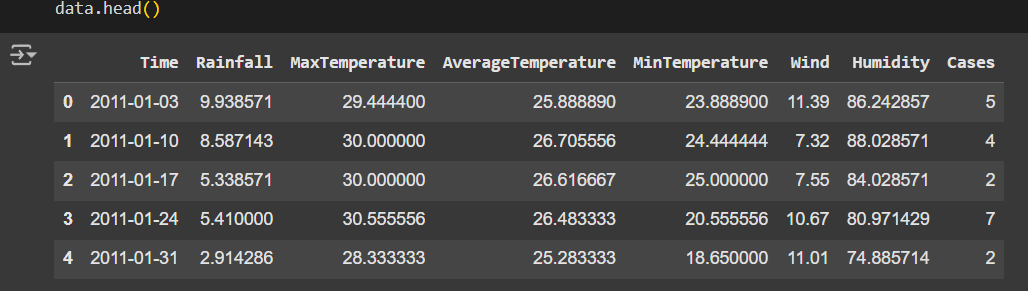
\includegraphics[width=0.75\textwidth]{data_snippet}
	\caption{Snippet of the Combined Dataset}
	\label{fig:data_snippet}
\end{figure}

\section{Preliminary Model Training}
The proposed Dengue Watch system utilized four distinct models to forecast weekly dengue cases: Long Short-Term Memory (LSTM) networks, Autoregressive Integrated Moving Average (ARIMA), Seasonal ARIMA (SARIMA), and Kalman Filter. Each model was trained on a dataset containing 452 weeks of historical dengue cases from 2016 to 2024, with meteorological variables such as temperature, humidity, and rainfall.

To optimize predictive performance, hyperparameter tuning was conducted individually for each model, refining parameters to achieve the most accurate and reliable forecasts. Following training, the models were rigorously evaluated against the dataset using a set of key performance metrics, including Mean Squared Error (MSE) and Root Mean Squared Error (RMSE).

The table below provides a summary and comparative analysis of each model’s results across these metrics, offering insights into the strengths and limitations of each forecasting technique for dengue case prediction in Iloilo City. 

\begin{table}[h!]
	\centering
	\begin{tabular}{|l|c|c|}
		\hline
		\textbf{Model} & \textbf{MSE} & \textbf{RMSE} \\ \hline
		\textbf{LSTM} & \textbf{342.59} & \textbf{18.51} \\ \hline
		\begin{tabular}[c]{@{}l@{}}\textbf{Seasonal ARIMA} \\ \textbf{(2, 0, 2) (0, 1,1)}\end{tabular} & \textbf{1198} & \textbf{34.62} \\ \hline
		\textbf{ARIMA (2, 0, 3)} & \textbf{1983.16} & \textbf{44.53} \\ \hline
		\textbf{Kalman Filter} & \textbf{2755.77} & \textbf{52.49} \\ \hline
	\end{tabular}
	\caption{Comparison of Models}
	\label{tab:comparison_of_models}
\end{table}

\subsection{LSTM Model}
The LSTM model architecture consisted of an input layer, a single LSTM layer with 64 units and ReLU activation, followed by a dense layer with a single output neuron to predict the dengue case count. Key hyperparameters included:
\begin{itemize}
	\item Window Size: 10 weeks, representing the time steps used in the sequence data for each prediction.
	\item Epochs: 50 epochs were used for training, balancing sufficient training time with computational efficiency.
	\item Batch Size: 1, allowing the model to process one sequence at a time, which is beneficial for small datasets but increases training time.
	\item Optimizer: The Adam optimizer was chosen for its adaptive learning capabilities and stability in training. A custom learning rate of 0.0001 was set to ensure gradual convergence and minimize risk of overfitting.
\end{itemize}

The dataset was split into training and test sets to evaluate the model’s performance and generalizability:
\begin{itemize}
	\item Training Set: 85\% of the data (385 sequences) was used for model training, enabling the LSTM to learn underlying patterns in historical dengue case trends and their relationship with weather variables.
	\item Test Set: The remaining 15\% of the data (67 sequences) was reserved for testing
\end{itemize}

Upon testing, the LSTM model produced an MSE of 342.59 and an RMSE of 18.51, showing its capability to generalize to unseen data. The close alignment of actual and predicted values in the test set plot supports this observation, suggesting that the model successfully captured critical temporal trends that correlate with dengue outbreaks.

\begin{figure}[H]
	\centering
	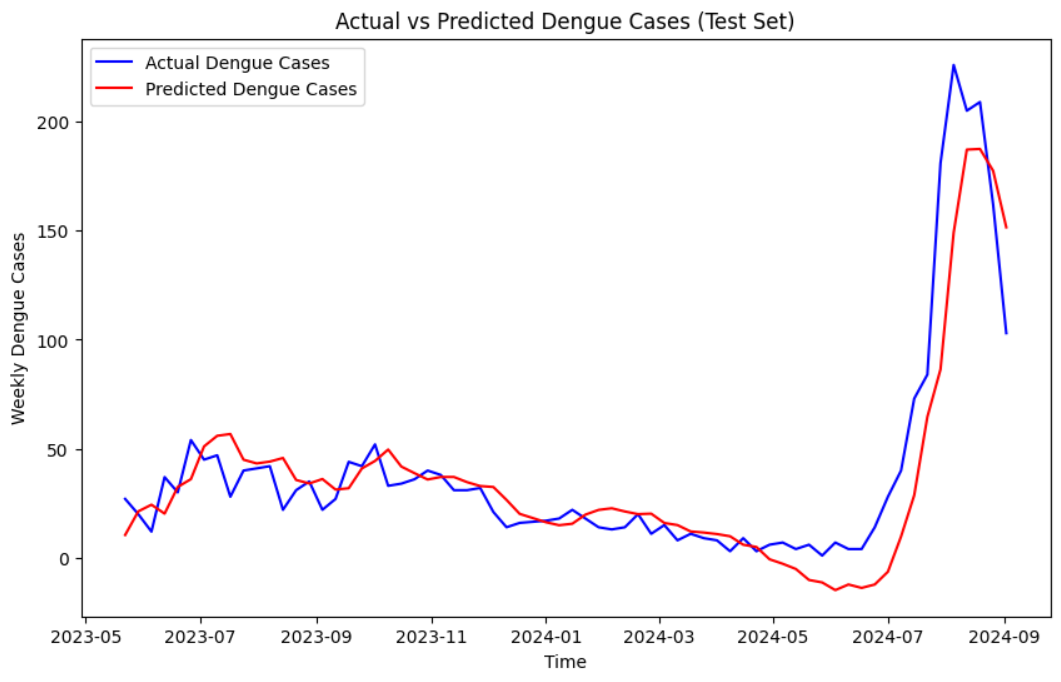
\includegraphics[width=1\textwidth]{line_graph_LSTM}
	\caption{LSTM Prediction Results for Test Set}
	\label{fig:LSTM_result}
\end{figure}

\subsection{ARIMA Model}

\begin{figure}[H]
	\centering
	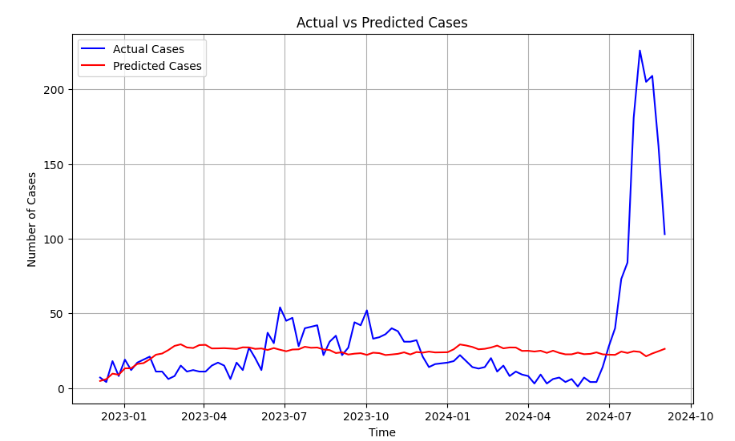
\includegraphics[width=1\textwidth]{line_graph_Arima}
	\caption{ARIMA Prediction Results for Test Set}
	\label{fig:Arima_result}
\end{figure}

\subsection{Seasonal ARIMA Model}

\begin{figure}[H]
	\centering
	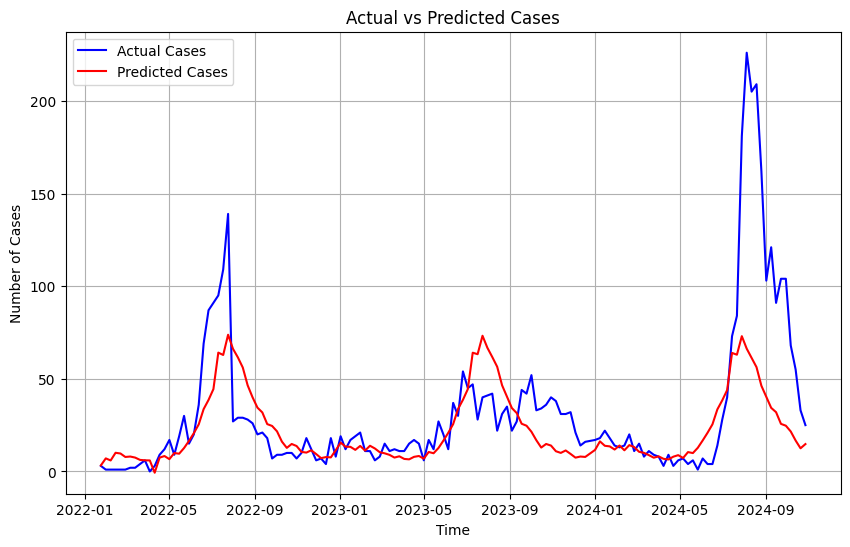
\includegraphics[width=1\textwidth]{line_graph_Sarima}
	\caption{Seasonal ARIMA Prediction Results for Test Set}
	\label{fig:Sarima_result}
\end{figure}

\subsection{Kalman Filter Model}

\begin{figure}[H]
	\centering
	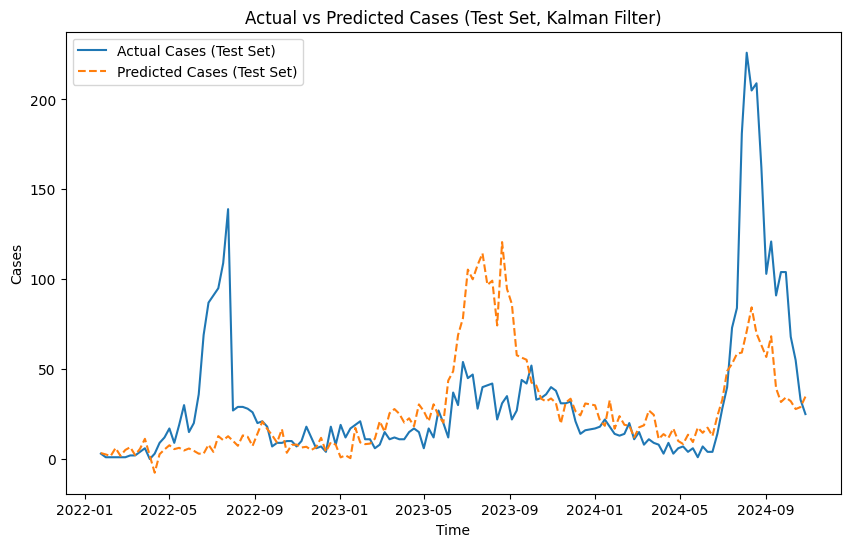
\includegraphics[width=1\textwidth]{line_graph_Kalman}
	\caption{Kalman Filter Prediction Results for Test Set}
	\label{fig:Kalman_result}
\end{figure}
\clearpage

\section{Guest Interface}

The Guest Interface is intended for all visitors of the web application. It shows the related statistics for dengue cases in a particular area and time. As the system is still in its testing phase, the data and charts shown in Figure 4.2 are generated from Python's Faker library. 

\begin{figure}[H]
	\centering
	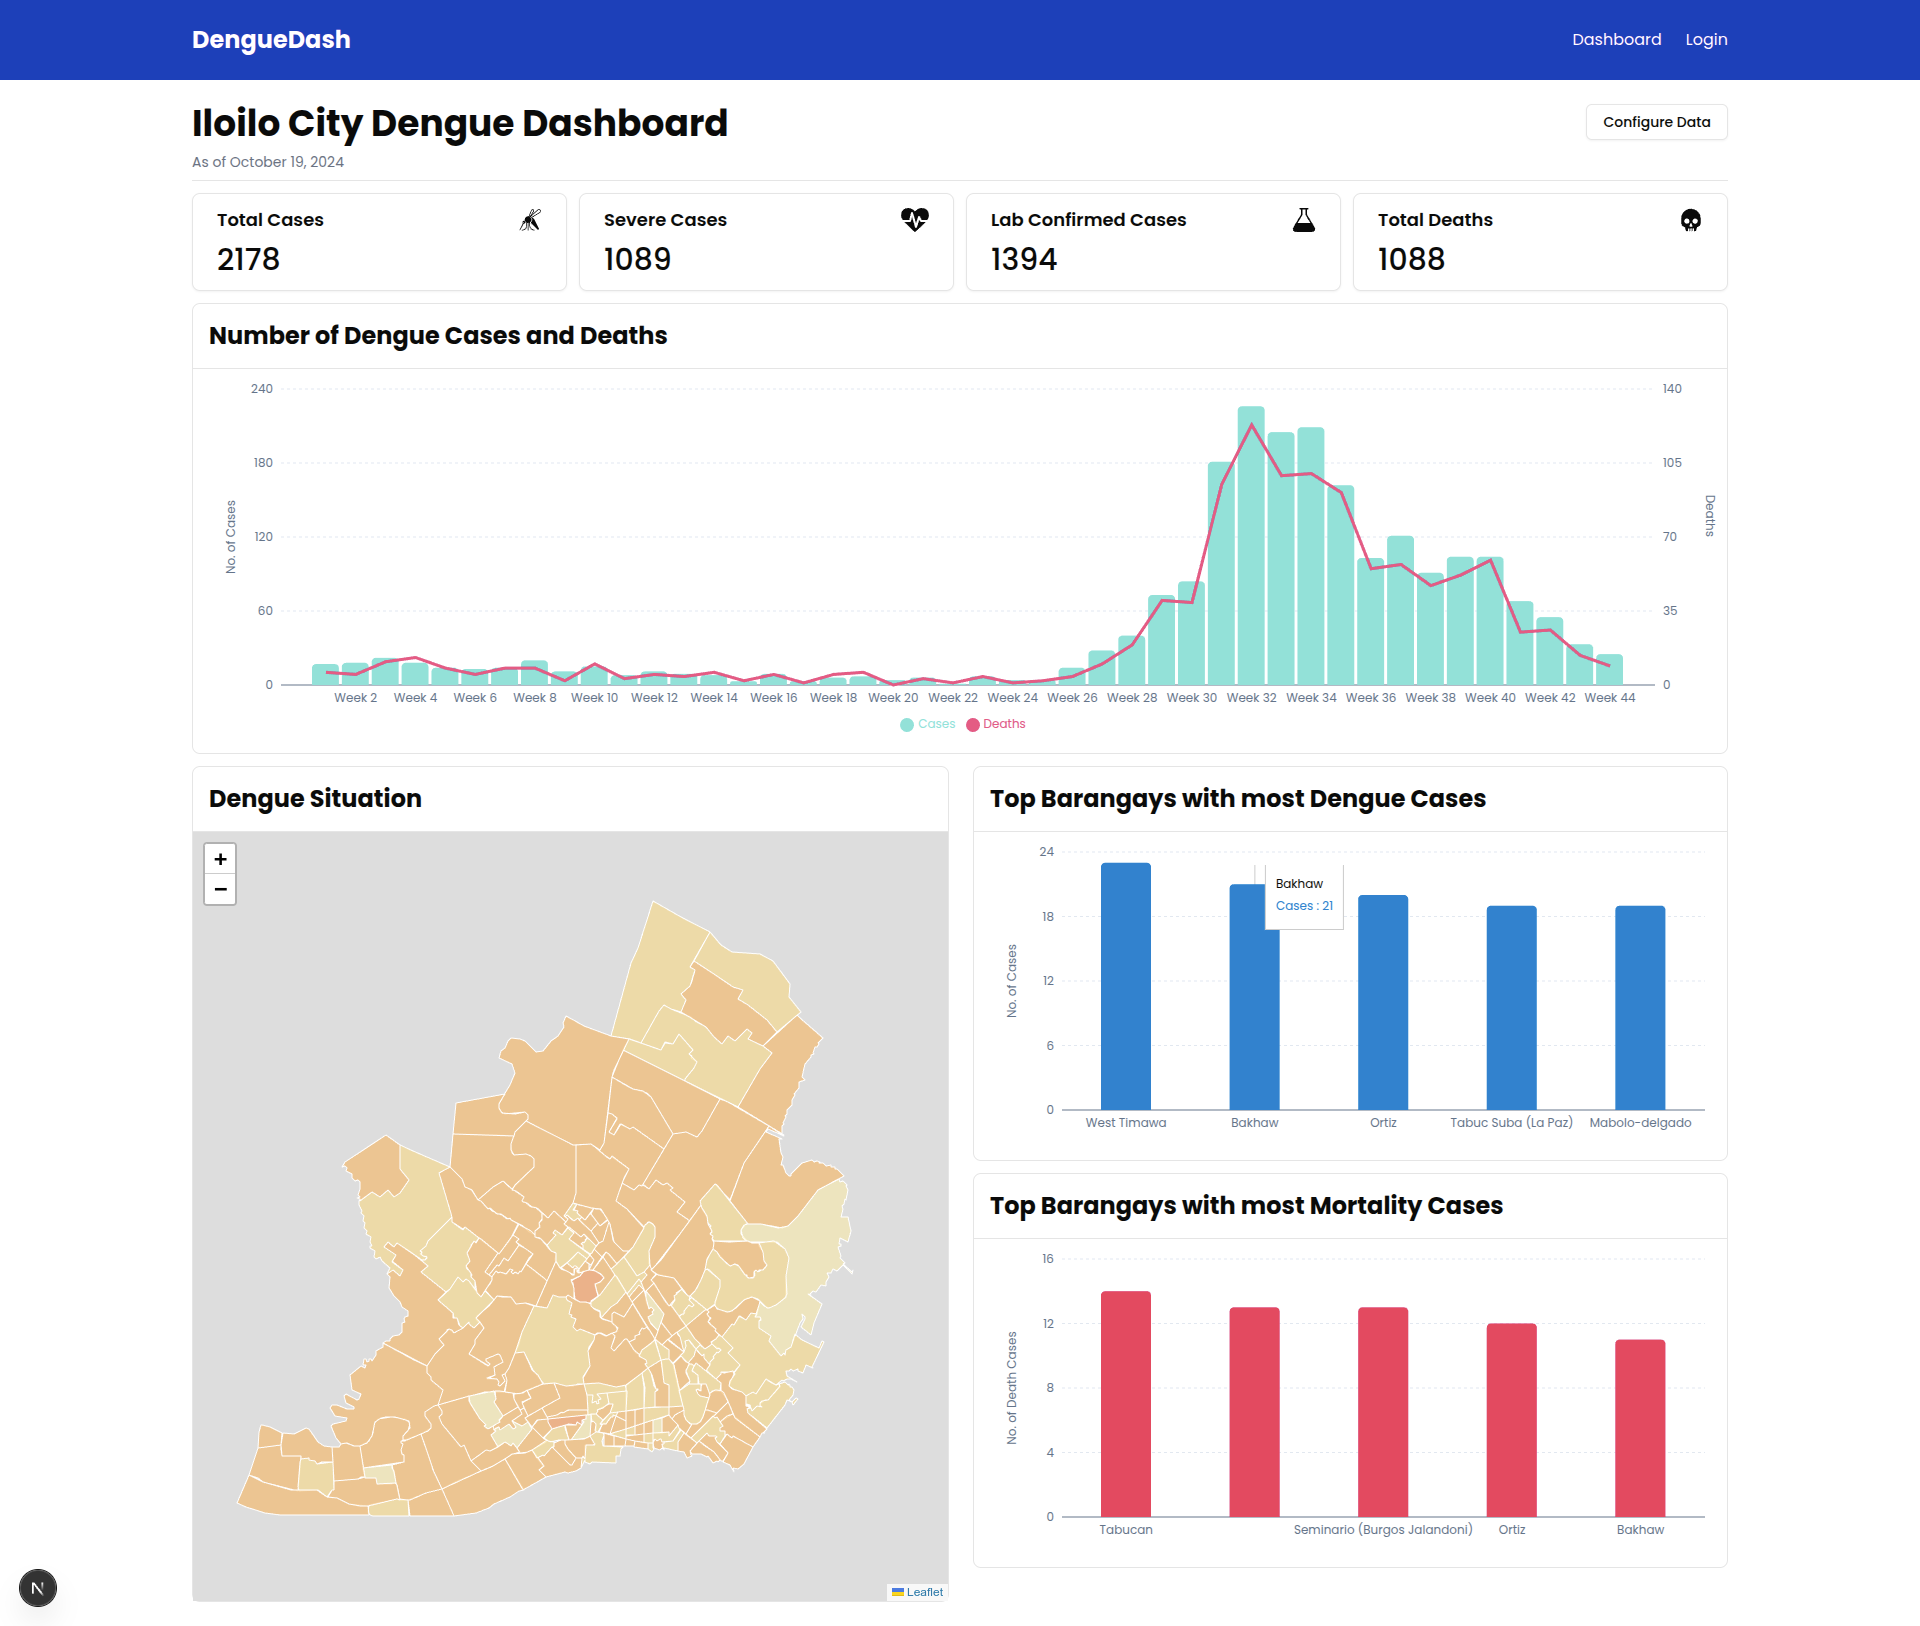
\includegraphics[width=1\textwidth]{guest_dashboard}
	\caption{Dashboard for Guests}
	\label{fig:guest_dashboard}
\end{figure}

\section{Personnel Interface}

\subsection{User Authentication, and Login}
To protect the data's integrity in production, it has been decided that the registration process will not be visible. Instead, an admin must register a user using a different interface. As of the moment, registering a user is done using API via Postman. In the login process, the system implements HTTP-only cookies that save the access token to protect against XSS attacks. After proper credentials have been provided, it will redirect to the user's home page.

\begin{figure}[H]
	\centering
	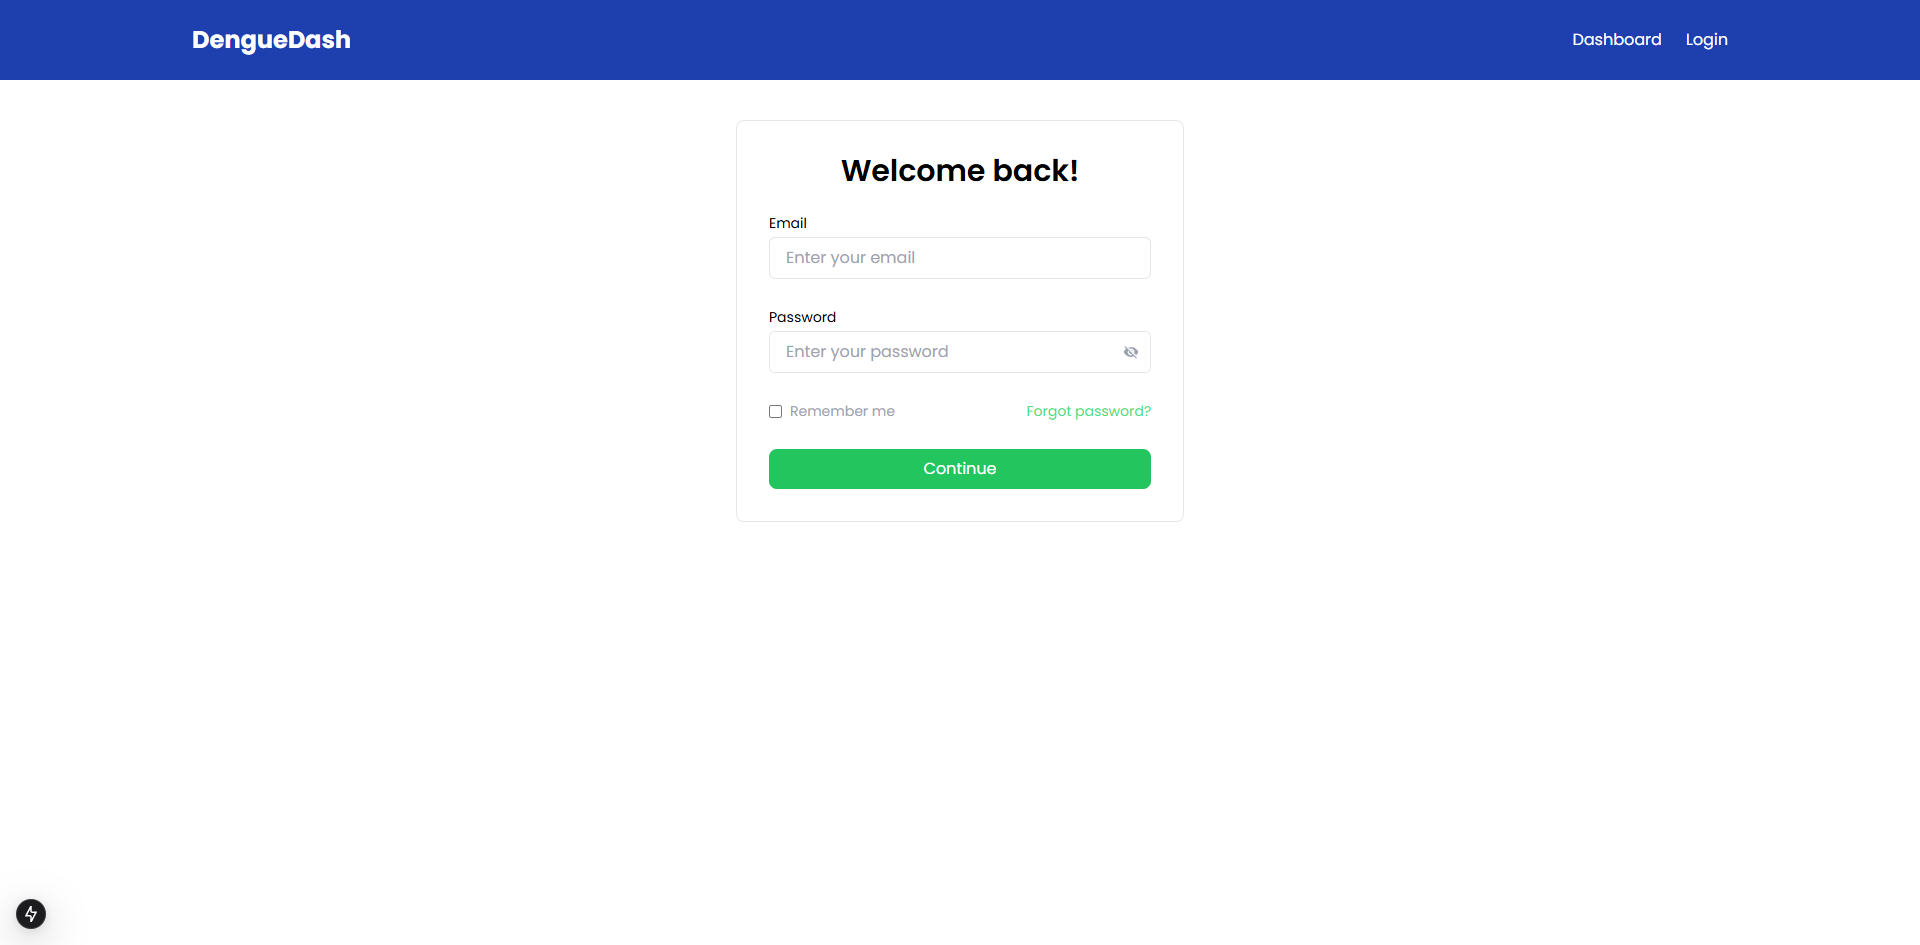
\includegraphics[width=1\textwidth]{login}
	\caption{Login Page for Users}
	\label{fig:login_page}
\end{figure}

\begin{figure}[H]
	\centering
	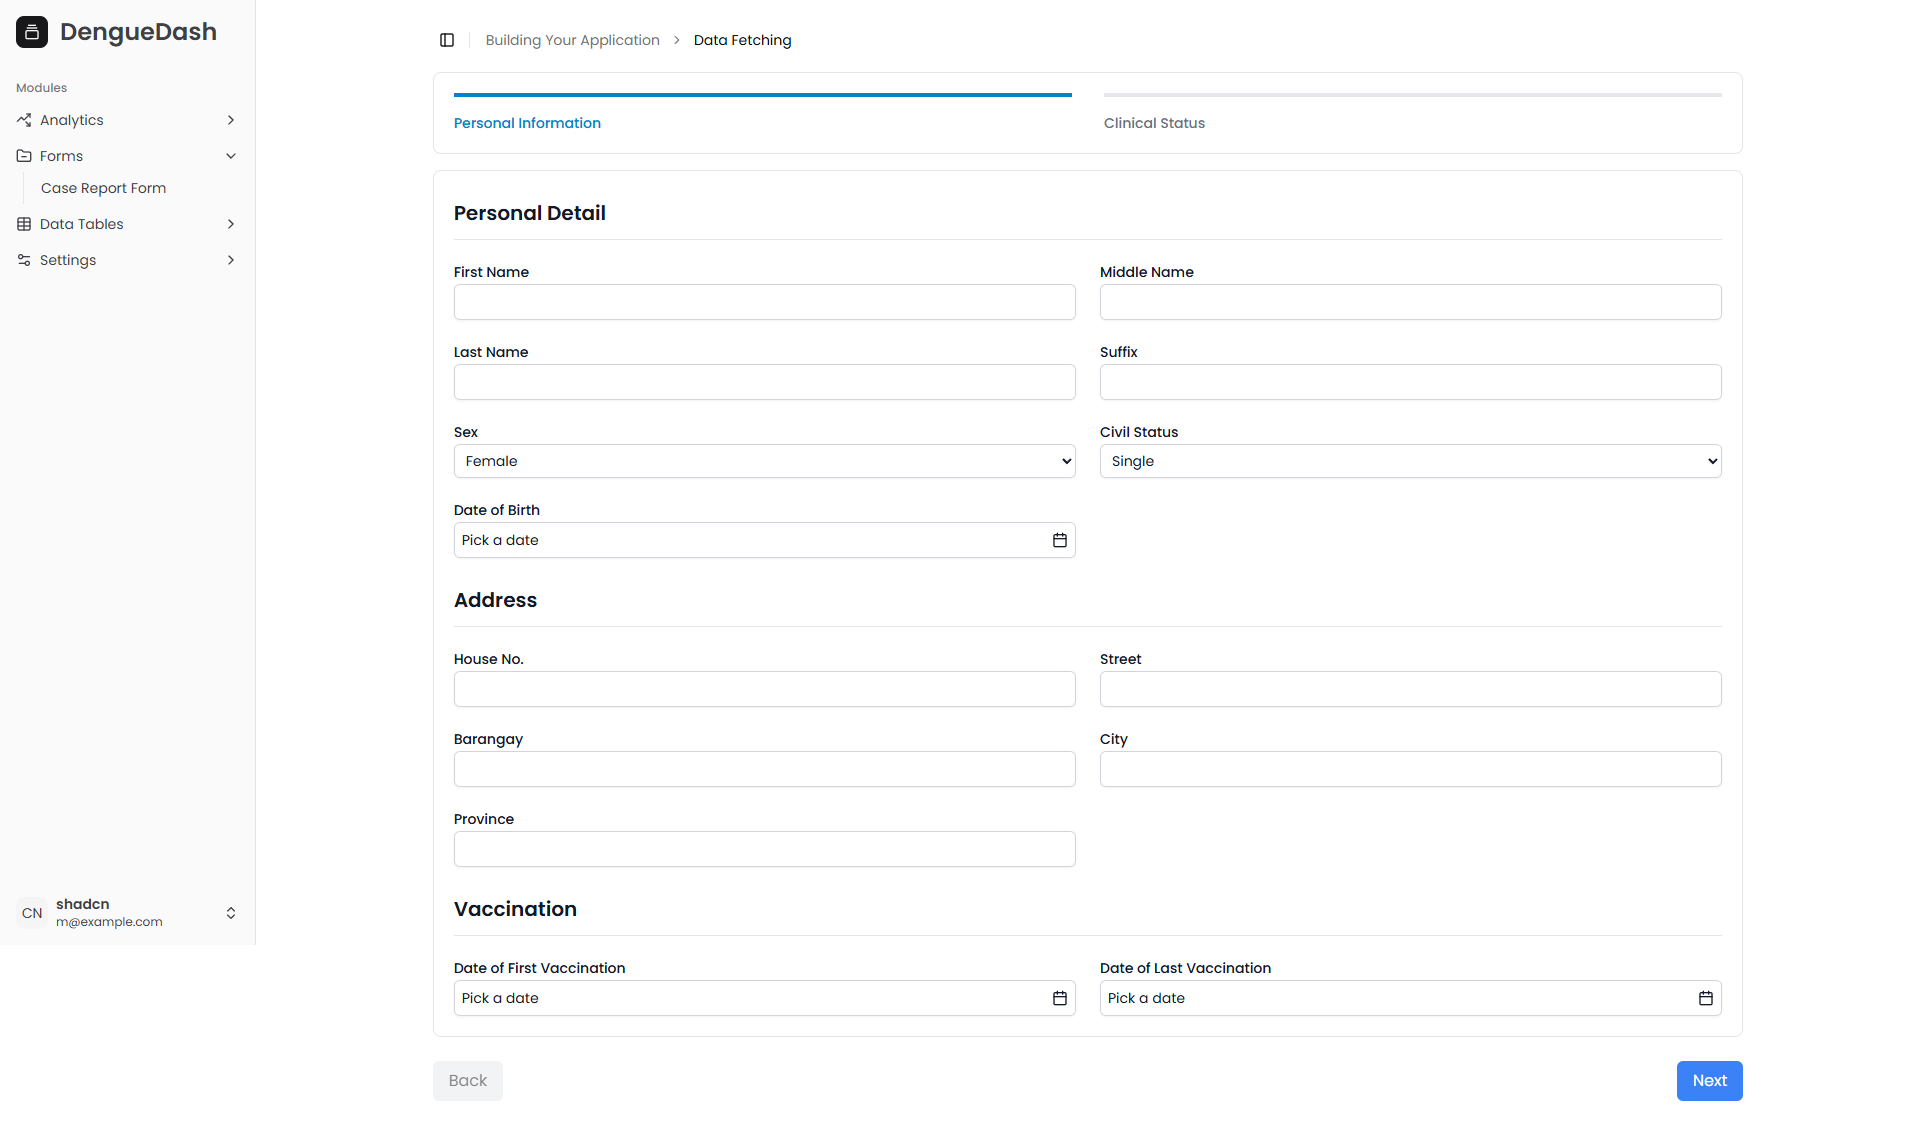
\includegraphics[width=1\textwidth]{case_report_form_1}
	\caption{First Part of Case Report Form}
	\label{fig:case_report_form_1}
\end{figure}

\begin{figure}[H]
	\centering
	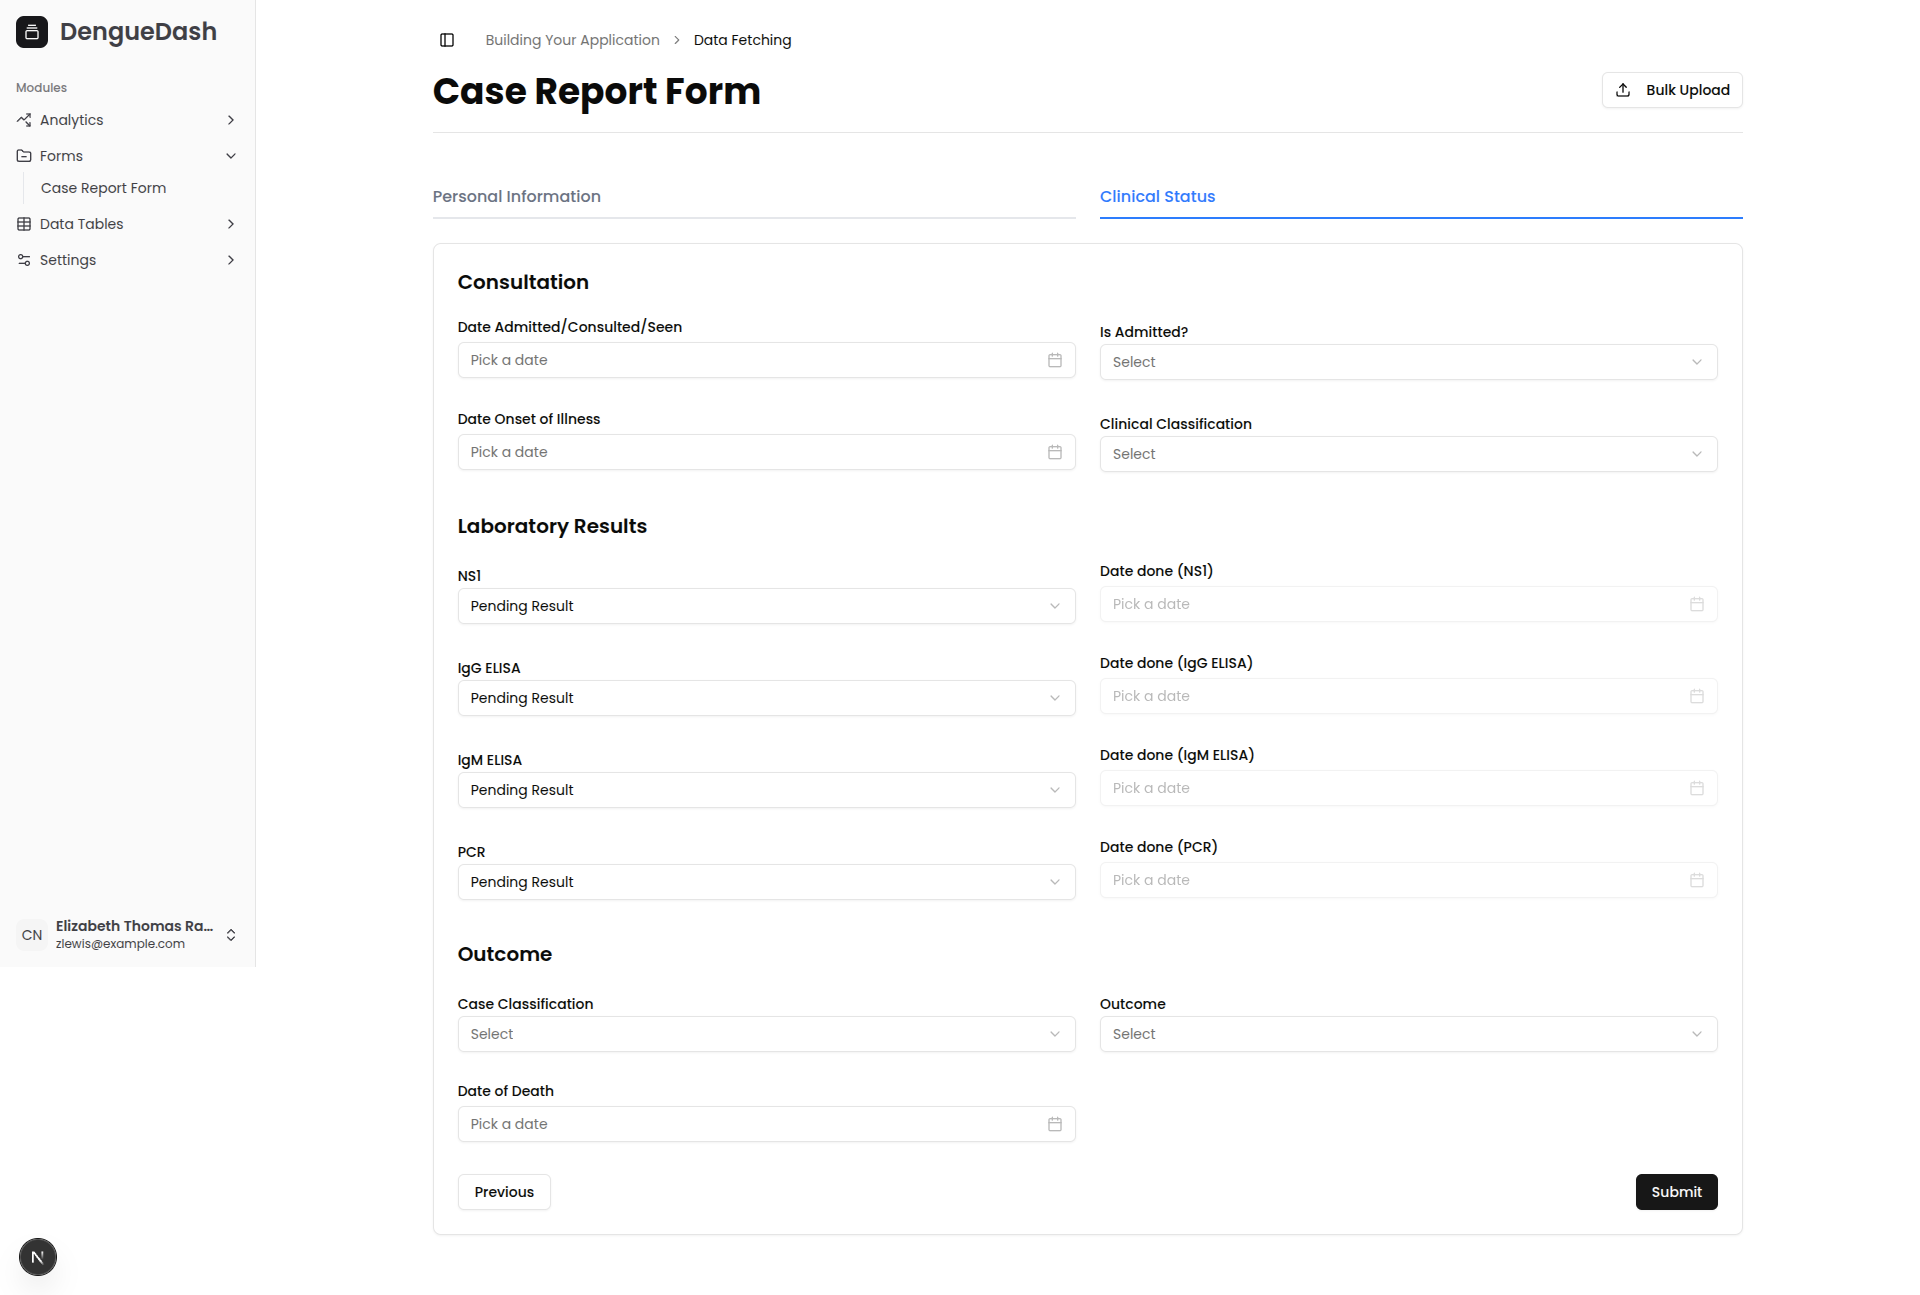
\includegraphics[width=1\textwidth]{case_report_form_2}
	\caption{Second Part of Case Report Form}
	\label{fig:case_report_form_2}
\end{figure}

\begin{figure}[H]
	\centering
	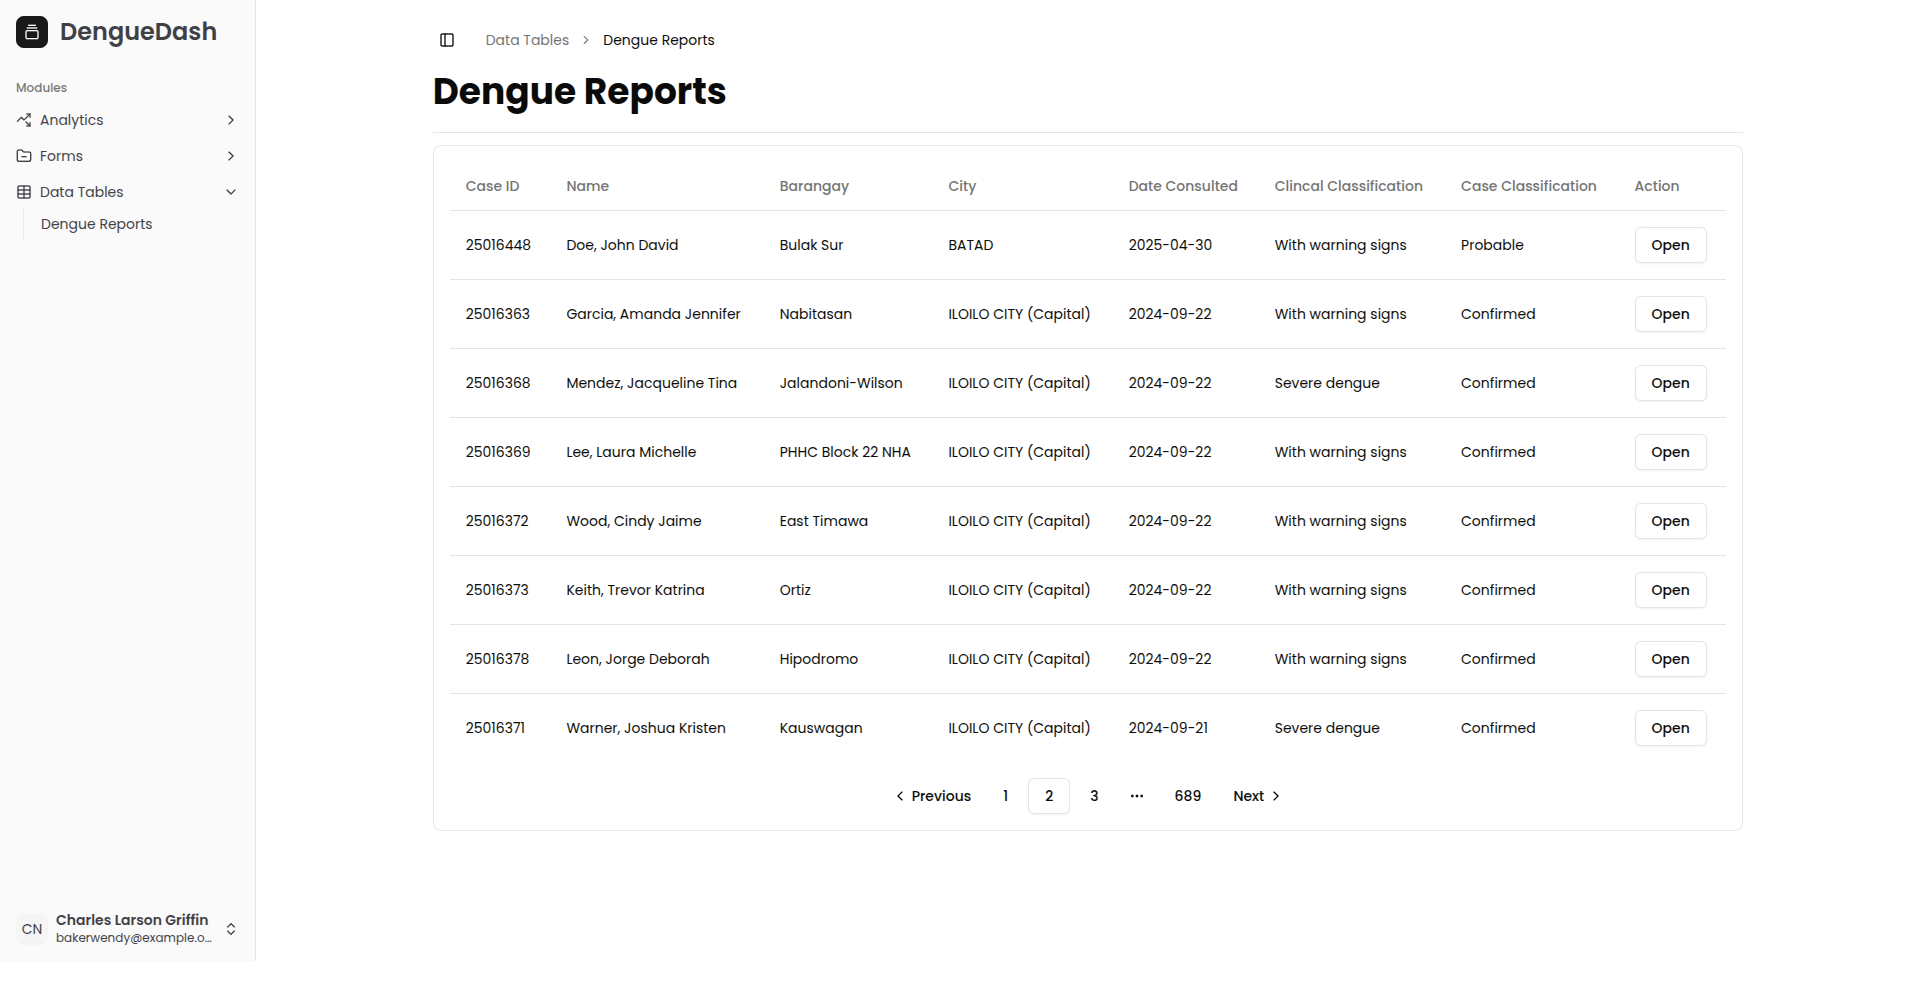
\includegraphics[width=1\textwidth]{dengue_reports}
	\caption{Dengue Reports}
	\label{fig:dengue_reports}
\end{figure}

